\documentclass{ltjsbook}
\usepackage{docmute} 
\usepackage{../../myStyle} 

\begin{document}
\chapter{多次元尺度法とその応用}
\label{H08_MDS}
% 10. MDS の展開　 → データの相と元，展開法，多次元展開法，個人差 MDS，非対称 MDS
多次元尺度構成法(MDS)は距離データから地図を作る方法であり，データに複雑なモデルを仮定しないためさまざまな適用例を考えることができます。
ここではその応用例をいくつかみていくことにします。

その前に，分析するデータの種類について新しい概念を導入します。

\section{データの相と元}
\label{ModeAndWay}
数値として得られたデータがどの程度の算術操作に耐えうるかについては，尺度水準によって分類できるのでした。
これとは別に，データがどのような要素の組み合わせでできているか，という観点から分類することがあります。それがデータの\keyterm{相}{そう}{mode}と\keyterm{元}{げん}{way}という区分です。

データの相とは，データを構成する要素の種類の数を指します。たとえばMDSで例に挙げた「都市間の距離」をみてみると，距離行列は都市$\times$都市のデータセットです。つまり要素の種類としては「都市」の一種類しかありません。このようなデータは一相のデータといいます。
あるいはまた，一般的な調査データを考えてみましょう。スプレッドシートに数値情報が並びますが，一般に一行に1ケース(個体，オブザベーション)，一列に1変数の矩形データです。これは個体$\times$変数なので，データを構成する要素は2つありますから，二相のデータといいます。
今度は追跡調査，つまり同じ人に複数回調査を行う例を考えてみましょう。スプレッドシートには「調査時期」という変数列が1つ増えただけと考えることもできますが，その中身は個体$\times$変数$\times$時点，という3つの要素から成り立っている3相データと考えることができます。
このように含まれる要素の(種類の)組み合わせであり，相は「そのまとまりから何らかの共通点がある」と考えて情報を探るべき側面という意味合いがあります。いろいろ複雑にしていくことはできますが，多くても3，4相ぐらいのデータセットまでになることが一般的です\footnote{筆者が今まで見たことのある多相データのなかでもっとも複雑なのはテレビの視聴調査に関するもので，個体$\times$変数$\times$放送時間帯$\times$ジャンルという4相のものでした。}。

相は要素の種類の数でしたが，これに対して，データの元とはその組み合わせ回数のことを意味します。最初の都市間距離のデータは一相ですが，都市と都市の組み合わせで距離が作られます。都市を二回使っているので2元データです。両者を合わせて一相二元データといいます。一般的な調査データの場合は，個体$\times$変数なので二相二元データ，追跡調査の場合は三相三元データということになります。
特殊な例ですが，家庭内での人間関係を把握するための調査を考えてみましょう。父，母，子からなる家族を対象に，「お父さんはお母さんのことをどのように考えていますか」，「お父さんはお子さんがお母さんのことをどう考えているとお思いですか」といった調査です。家族構成員ひとりにつき，「父・母・子が」「父・母・子に対して」どのように考えているか，ということを尋ねますので，構成員$\times$父母子$\times$父母子の二相三元データということができます。
ここで，評価する主体と評価される客体は同一人物であっても異なる側面である，と考えることもできましょう。その場合は，構成員$\times$主体$\times$客体と考えて三相三元データになります。

つまり，相とは「その側面の特殊性・特徴を取り出して分析したい」と研究者が注目したい側面であって，同じデータであってもどのような情報を取り出すか，どこに情報が潜んでいるとみなすかによって扱いが変わるということです。
一般的な調査で，因子分析をするプロセスの最初に$\bm{R} = 1/n\bm{Z'Z}$という計算がありました。これはつまり回答者の相を要約して潰し，変数の相だけの一相二元データ(変数$\times$変数)に作り替えたことを意味します。もし個人の情報が重要であると考えるなら，個人の相から直接情報を取り出すことを考えるのも良いことかもしれません。\keyterm{構造方程式モデリング}{こうぞうほうていしきもでりんぐ}{Structural Equation Modeling}などを使って，注目したい相に含まれる潜在変数を仮定することで考察の光を当てることができます\footnote{手前ミソながら具体例として\textcite{kosugi2011}を挙げておきます。}。

皆さんもデータの分析にあたって，どの側面のどの情報を重要とみなすか，あるいはどの情報であれば要約可能であると考えられるかに，少し配慮してみてください。

\section{非計量多次元尺度法}

さて前章では，一相二元データの代表例である距離データをつかって，クラスター分析やMDSによって分類したり可視化したりできるということを見てきました。
ただし，この場合の距離行列とは，間隔尺度水準以上であることが必要なのでした。
しかし心理学的な刺激に対する反応をデータ化する時は，同時に被験者はそこまで鋭敏に反応しているのか，いいかえれば本当に間隔尺度水準以上の精度で判断できているのかな，という人間側の問題が気になりますね。そこまで人間は鋭敏な反応をしていないかもしれません。

数値的な厳密さを持つデータのことを\keyterm{計量}{けいりょう}{metric}データと呼ぶことがありますが，人文社会科学的なデータはせいぜい順序尺度程度の違いしかもたない\keyterm{非計量}{ひけいりょう}{non-metric}データです。この非計量データを加工して，数値的特性を取り出そうとしても，元の数字に信憑性がないのですから結果も推して知るべしです。

でも大丈夫。MDSには非計量データに対応したものがあるのです。\keyterm{非計量的多次元尺度構成法}{ひけいりょうてきたじげんしゃくどこうせいほう}{Non-Metric Multi-Dimensional Scaling}と呼ばれる手法がそれです。非計量MDSでは，対象$j$と$k$の類似度を$\delta_{jk}$とし，分析によって埋め込む多次元空間での距離を$d_{jk}$としたときに，次の関係が保持されることだけを考えます\footnote{一般的な統計の文脈では，推定値をギリシア文字で，実測値をアルファベットで表記する習わしですが，MDSの文脈では逆に仮想空間の値・座標をアルファベットで，生データによる測定値をギリシア文字で表現することが一般的です。なんでだろう。}。

$$ \delta_{jk} > \delta_{lm} \mbox{ならば}d_{jk}\le d_{lm} $$

これは評定値のような非計量データの世界を参考に，距離関係が保持されている仮想的・理論的な空間を作ってそこでの布置を考えようというモデルです。評定の世界と構成される世界が(対応関係はあるものの)別立てになっているところに注目してください。

多次元空間をどのように構成するかについては，埋め込まれる空間での距離$d_{jk}$を配置する仮想空間上での，推定される距離$\hat{d}_{jk}$の差の二乗和，特に
\[ stress = \sqrt{\frac{\sum \sum_{j\neq k}(\hat{d}_{jk}-d_{jk})^2}{\sum \sum d_{jk}^2}} \]
が最小になるように，反復計算で座標を求めていくのが古典的なKruscalの方法とよばれているものです\parencite{kruskal1964}。ここで定義した不適合度は特に\keyterm{ストレス}{すとれす}{Stress}と呼ばれ，Kuruscalの提案の他にもいくつかの方法が考えられています。
このストレス値が小さければ小さいほど，データと埋め込まれた空間の差が小さい，つまり当てはまりが良いと考えるのです。

非計量MDSはRの\verb|MASS|パッケージや\verb|smacof|パッケージに実装されており，簡単に試すことができます。具体例で見てみましょう。

\subsection{非計量多次元尺度法の例}

ここでは\verb|MASS|パッケージに含まれる\verb|isoMDS|関数を使って実践してみます。

使うデータは，2021年末のM-1グランプリの評定をデータ化したものです\footnote{念のために解説しておきますが，M-1グランプリとは2001年から始まった漫才の賞レースの1つで，年末に年間チャンピオンが決定します。開催年ごとにルールが少し変わることもありますが，基本的には予選を勝ち抜いた10組の漫才師が4分間のネタを披露し，6-7名の審査員が100点満点で採点します。点数の上位3組が決勝戦を行い2本目のネタを披露，投票によりチャンピオンが選出されるという流れです。2021年はオール巨人，富澤たけし，塙宣之，立川志らく，中川礼二，松本人志，上沼恵美子が審査員で，最終的には錦鯉がチャンピオンになりました。このデータセットは1本目のネタについての採点を2001年から集めたものになります。}。2021年度のスコアは表\ref{tbl:h15_m1}にあるようなものでした

\begin{table}[ht]
	\centering
	\caption{M-1グランプリ2021の採点結果}
	\begin{tabular}{l|cccccccc}
		\hline
		演者        & 巨人 & 富澤 & 塙  & 志らく & 礼二 & 松本 & 上沼 \\
		\hline
		モグライダー    & 91 & 93 & 92 & 89  & 90 & 89 & 93 \\
		ランジャタイ    & 87 & 91 & 90 & 96  & 89 & 87 & 88 \\
		ゆにばーす     & 89 & 92 & 91 & 91  & 93 & 88 & 94 \\
		ハライチ      & 88 & 90 & 89 & 90  & 89 & 92 & 98 \\
		真空ジェシカ    & 90 & 89 & 92 & 94  & 94 & 90 & 89 \\
		オズワルド     & 94 & 95 & 95 & 96  & 96 & 96 & 93 \\
		ロングコートダディ & 89 & 90 & 93 & 95  & 95 & 91 & 96 \\
		錦鯉        & 92 & 94 & 94 & 90  & 96 & 94 & 95 \\
		インディアンス   & 92 & 91 & 93 & 94  & 94 & 93 & 98 \\
		もも        & 91 & 90 & 91 & 96  & 95 & 92 & 90 \\
		\hline
	\end{tabular}
	\label{tbl:h15_m1}
\end{table}


M-1の採点は審査員各自の主観に基づいて行われ，得点の絶対値はそれほど重要ではないかもしれません。すなわち，松本人志の80点が上沼恵美子の80点と同じぐらいの面白さを評価しているか，ということについては真偽判断ができないでしょう。それでも各審査員の中での相対的評価には，一貫性がありそうです。すなわちある審査員が漫才師Aに80点，漫才師Bに85点をつけたのならBの方が面白かったということでしょうし，漫才師Cが83点なら$A<C<B$という順序はあると思われます。つまり\keytermL{順序尺度水準}{じゅんじょしゃくどすいじゅん}程度の質はあると仮定することに無理はなさそうです。

そこでこのデータをもとに，10組の漫才師の類似度を計算します。類似度はユークリッド距離を用いることにします。ユークリッド距離は既に述べたように差分の二乗を総和して平方根を取ったものですが，具体的な数字で見た方がわかりやすいかもしれませんので，表\ref{tbl:h15_distance}を用意しました。
\begin{table}[ht]
	\centering
	\caption{距離の計算}
	\begin{tabular}{l|rrrrrrrr}
		\hline
		       & 巨人 & 富澤 & 塙  & 志らく & 礼二 & 松本 & 上沼 & 総和  \\
		\hline
		モグライダー & 91 & 93 & 92 & 89  & 90 & 89 & 93 & 637 \\
		ランジャタイ & 87 & 91 & 90 & 96  & 89 & 87 & 88 & 628 \\
		\hline
		差分     & 4  & 2  & 2  & -7  & 1  & 2  & 5  & 9   \\
		差分の二乗  & 16 & 4  & 4  & 49  & 1  & 4  & 25 & 103 \\
		\hline
	\end{tabular}
	\label{tbl:h15_distance}
\end{table}
表\ref{tbl:h15_distance}にモグライダーとランジャタイの二組だけ取り出し，これで計算例を見てみます。それぞれの得点の差分，その二乗を計算し，それを総和したところ$103$という値になっています。これの平方根を取ったもの，すなわち$\sqrt{103}=10.14889$がこの二組の距離，すなわち非類似度ということになります。この計算を全ての組み合わせについて計算してくれるのが，\verb|dist|関数なのです。

\begin{lstlisting}[language=C++,label={code:x15_02},caption={距離行列の計算}]
dat <- read_csv("M1score2021.csv")
dat.mat <- dat %>%
  dplyr::filter(年代 == 21) %>%
  arrange(ネタ順) %>% 
  dplyr::select(-年代, -ネタ順) %>%
  pivot_longer(-演者) %>%
  na.omit() %>%
  pivot_wider(id_cols = 演者, 
  			  names_from = name,
			  values_from = value) %>%
  as.matrix()
rownames(dat.mat) <- dat.mat[, 1]
dat.mat <- dat.mat[, -1] %>%
  dist()
\end{lstlisting}

\paragraph{コード解説}
\begin{description}
	\item[1行目] データファイルを読み込み，\verb|dat|オブジェクトに格納します\footnote{このデータセットは伴走サイト，\url{https://kosugitti.github.io/psychometrics_syllabus/}にサンプルデータとし置いてあります。}。
	\item[2-9行目] 必要なデータだけに絞り込む操作です。流れを解説しますが，他のやり方でもいいですしできあがったものが何かだけわかれば結構です。
	      \begin{description}
		      \item[3行目] 2021年のデータだけに絞り込みます。
		      \item[4行目] ネタ順に並び替えています。
		      \item[5行目] 年代変数とネタ順変数はもういらないので削除してしまっています。
		      \item[6行目] ロング型に変換しています。これで演者-審査員-採点のデータセットができます。
		      \item[7行目] 欠損値を除外しています。実はこれがこの操作の目的で，というのも過去の審査データも入っているものですから，過去の審査員も大量に変数として含まれていて，それらが欠損値になってしまっていたのです。
		      \item[8-10行目] 元のワイド型に戻しています。
		      \item[11行目] 以下の行列処理のため，\verb|data.frame|型から\verb|matrix|型に変換しています。
	      \end{description}
	\item[12行目] 変数として一列目に演者名が入っていますが，これを行列の行名に入れています。\verb|matrix|型は行名・列名をデータの外に持つのです。
	\item[13-14行目] 変数としての演者名を除いて，パイプで\verb|dist|関数に入れ，距離行列を作っています。
\end{description}
できた距離行列は，表\ref{tbl:h15_distMat}のようになっています。モグライダーとランジャタイの距離が，先ほどの例で計算した値と一致していることを確認してください。

\begin{table}[ht]
	\centering
	\caption{演者の非類似度行列(演者名は略記)}
	\begin{tabular}{l|ccccccccccc}
		\hline
		    & モグ     & ラン     & ゆに     & ハラ     & 真空     & オズ    & ロン    & 錦鯉    & インデ   & もも    \\
		\hline
		モグ  & 0.000  &        &        &        &        &       &       &       &       &       \\
		ラン  & 10.149 & 0.000  &        &        &        &       &       &       &       &       \\
		ゆに  & 4.583  & 9.165  & 0.000  &        &        &       &       &       &       &       \\
		ハラ  & 7.937  & 12.806 & 7.616  & 0.000  &        &       &       &       &       &       \\
		真空  & 8.660  & 7.483  & 7.071  & 11.832 & 0.000  &       &       &       &       &       \\
		オズ  & 12.490 & 15.652 & 12.207 & 14.933 & 11.000 & 0.000 &       &       &       &       \\
		ロン  & 9.381  & 11.446 & 6.403  & 9.110  & 7.416  & 9.487 & 0.000 &       &       &       \\
		錦鯉  & 8.485  & 15.264 & 8.307  & 10.909 & 10.247 & 7.071 & 7.874 & 0.000 &       &       \\
		インデ & 9.381  & 14.107 & 8.062  & 8.660  & 9.950  & 8.124 & 4.472 & 6.325 & 0.000 &       \\
		もも  & 10.100 & 9.110  & 8.307  & 12.207 & 3.606  & 8.718 & 6.782 & 9.592 & 8.718 & 0.000 \\
		\hline
	\end{tabular}
	\label{tbl:h15_distMat}
\end{table}
あとはこの距離行列を\verb|isoMDS|関数に渡すだけです。\verb|isoMDS|関数は引数として，何次元の解を求めるかを設定できます。地理データであれば2,3次元から作られていることは明らかですが，この評価が何次元かは事前にわかりません。
そこで次元数を1から7まで変化させながら，Stress値がどうなるかを表したのが図\ref{fig::15_02}になります\footnote{どうして7までか，というと評定者が7名だからです。7名それぞれの評価次元があると考えると，この距離空間の中には最大7次元あるはずですから。あるいは10組の演者がいますから，組み合わせの自由度から考えて9次元まで試してもいいと思います。}。

\begin{figure}[ht]
	\begin{center}
		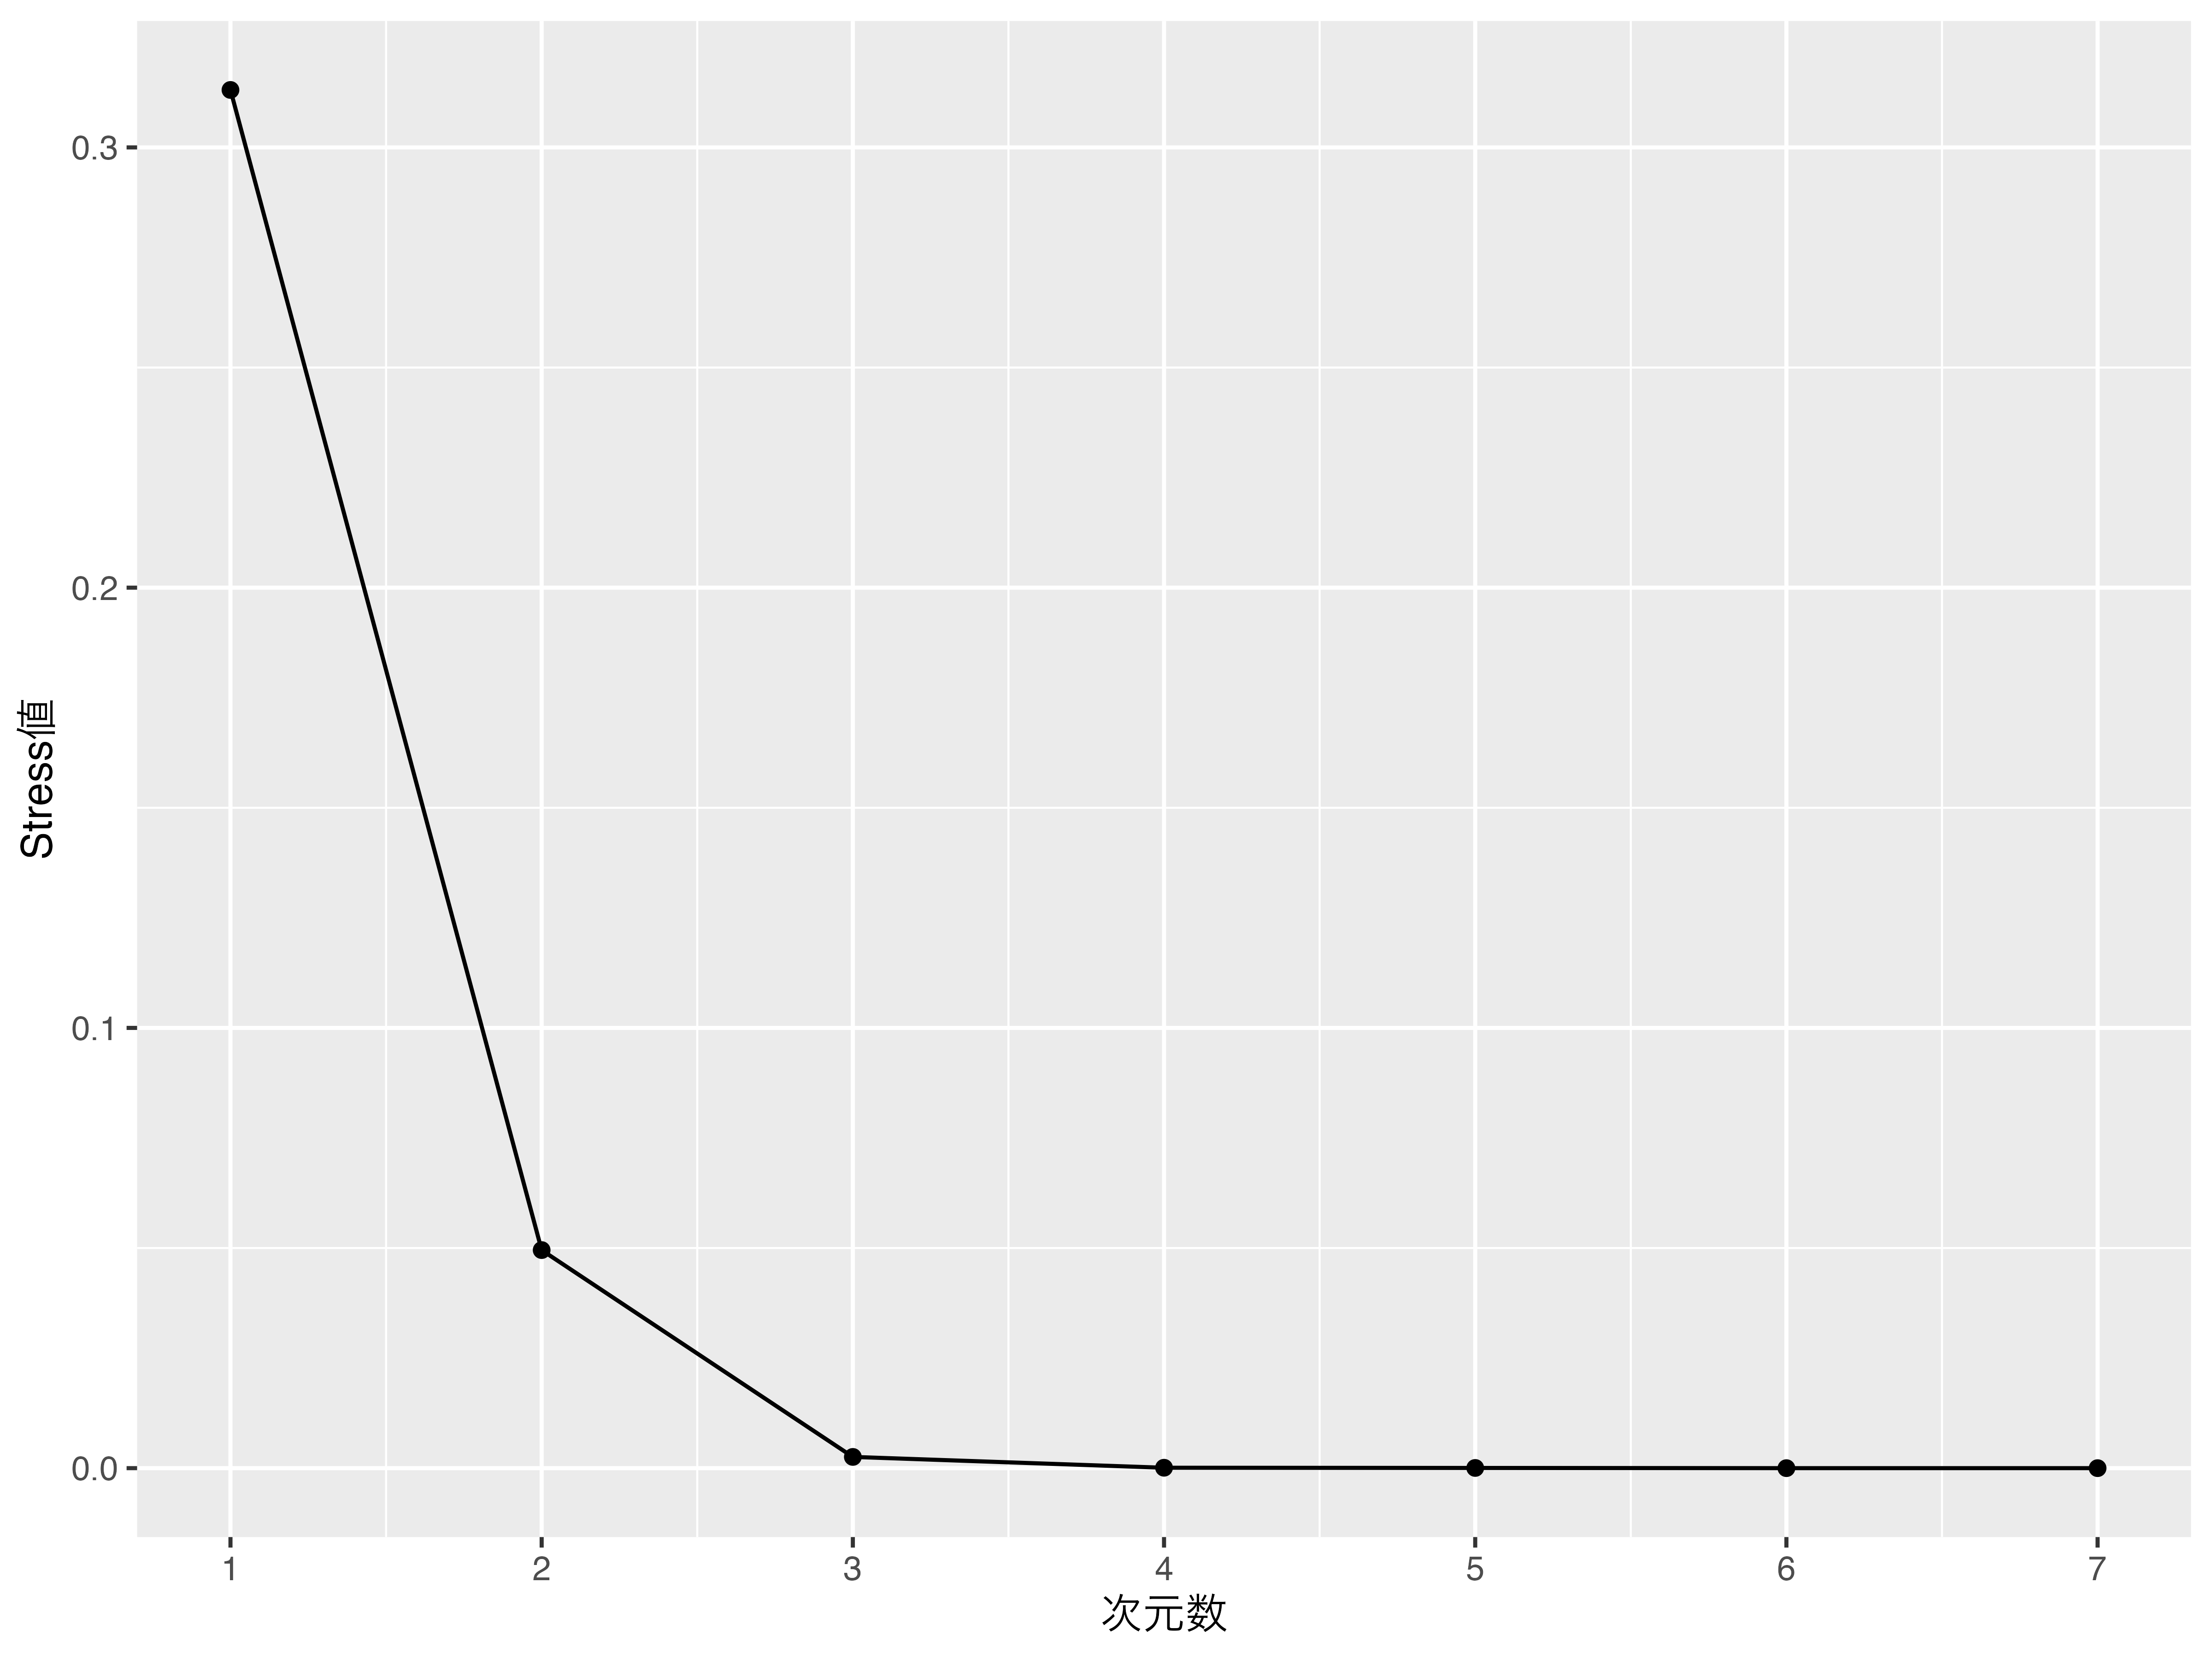
\includegraphics[width=0.8\linewidth,keepaspectratio]{../images/Rplot15_02.png}
		\caption{Stress値の減衰}
		\label{fig::15_02}
	\end{center}
\end{figure}

まるで因子分析の\keytermL{スクリープロット}{すくりーぷろっと}のようですね。横軸に次元数，縦軸にStress値を置いた折れ線グラフですが，当然のことながら反映させるMDS空間の次元数が増えるとデータとの距離が縮んでいきます。
\textcite{kruskal1964multidimensional}の基準によれば，Stress値は表\ref{tbl:x15_stress}のように評価できます。この基準でいくと，今回は2次元で4.9\%(0.0049534)ですから，2次元解でOKとしましょう。

\begin{table}[ht]
	\centering
	\caption{Stress値の評価}
	\begin{tabular}{cc}
		Stress           & Goodness of Fit \\\hline
		20\%             & poor            \\
		10\%             & fair            \\
		5\%              & good            \\
		$2\frac{1}{2}$\% & excellent       \\
		0\%              & ``perfect''     \\\hline
	\end{tabular}
	\label{tbl:x15_stress}
\end{table}

演者をプロットしたのが図\ref{fig::15_03}です。東西南北というか，上下左右の軸に特に意味はありませんから，因子分析のように因子軸の解釈や命名をすることはありません。近くにプロットされた対象は評価が似ていたんだな，ということがわかりますし，相対的な位置関係から，「ハライチとももは芸風が真逆だな」とか「ロングコートダディは中心に近いから中庸的な笑い，悪く言えばキャラが立ってないんだな」といったことが読み取れます。
\begin{figure}[ht]
	\begin{center}
		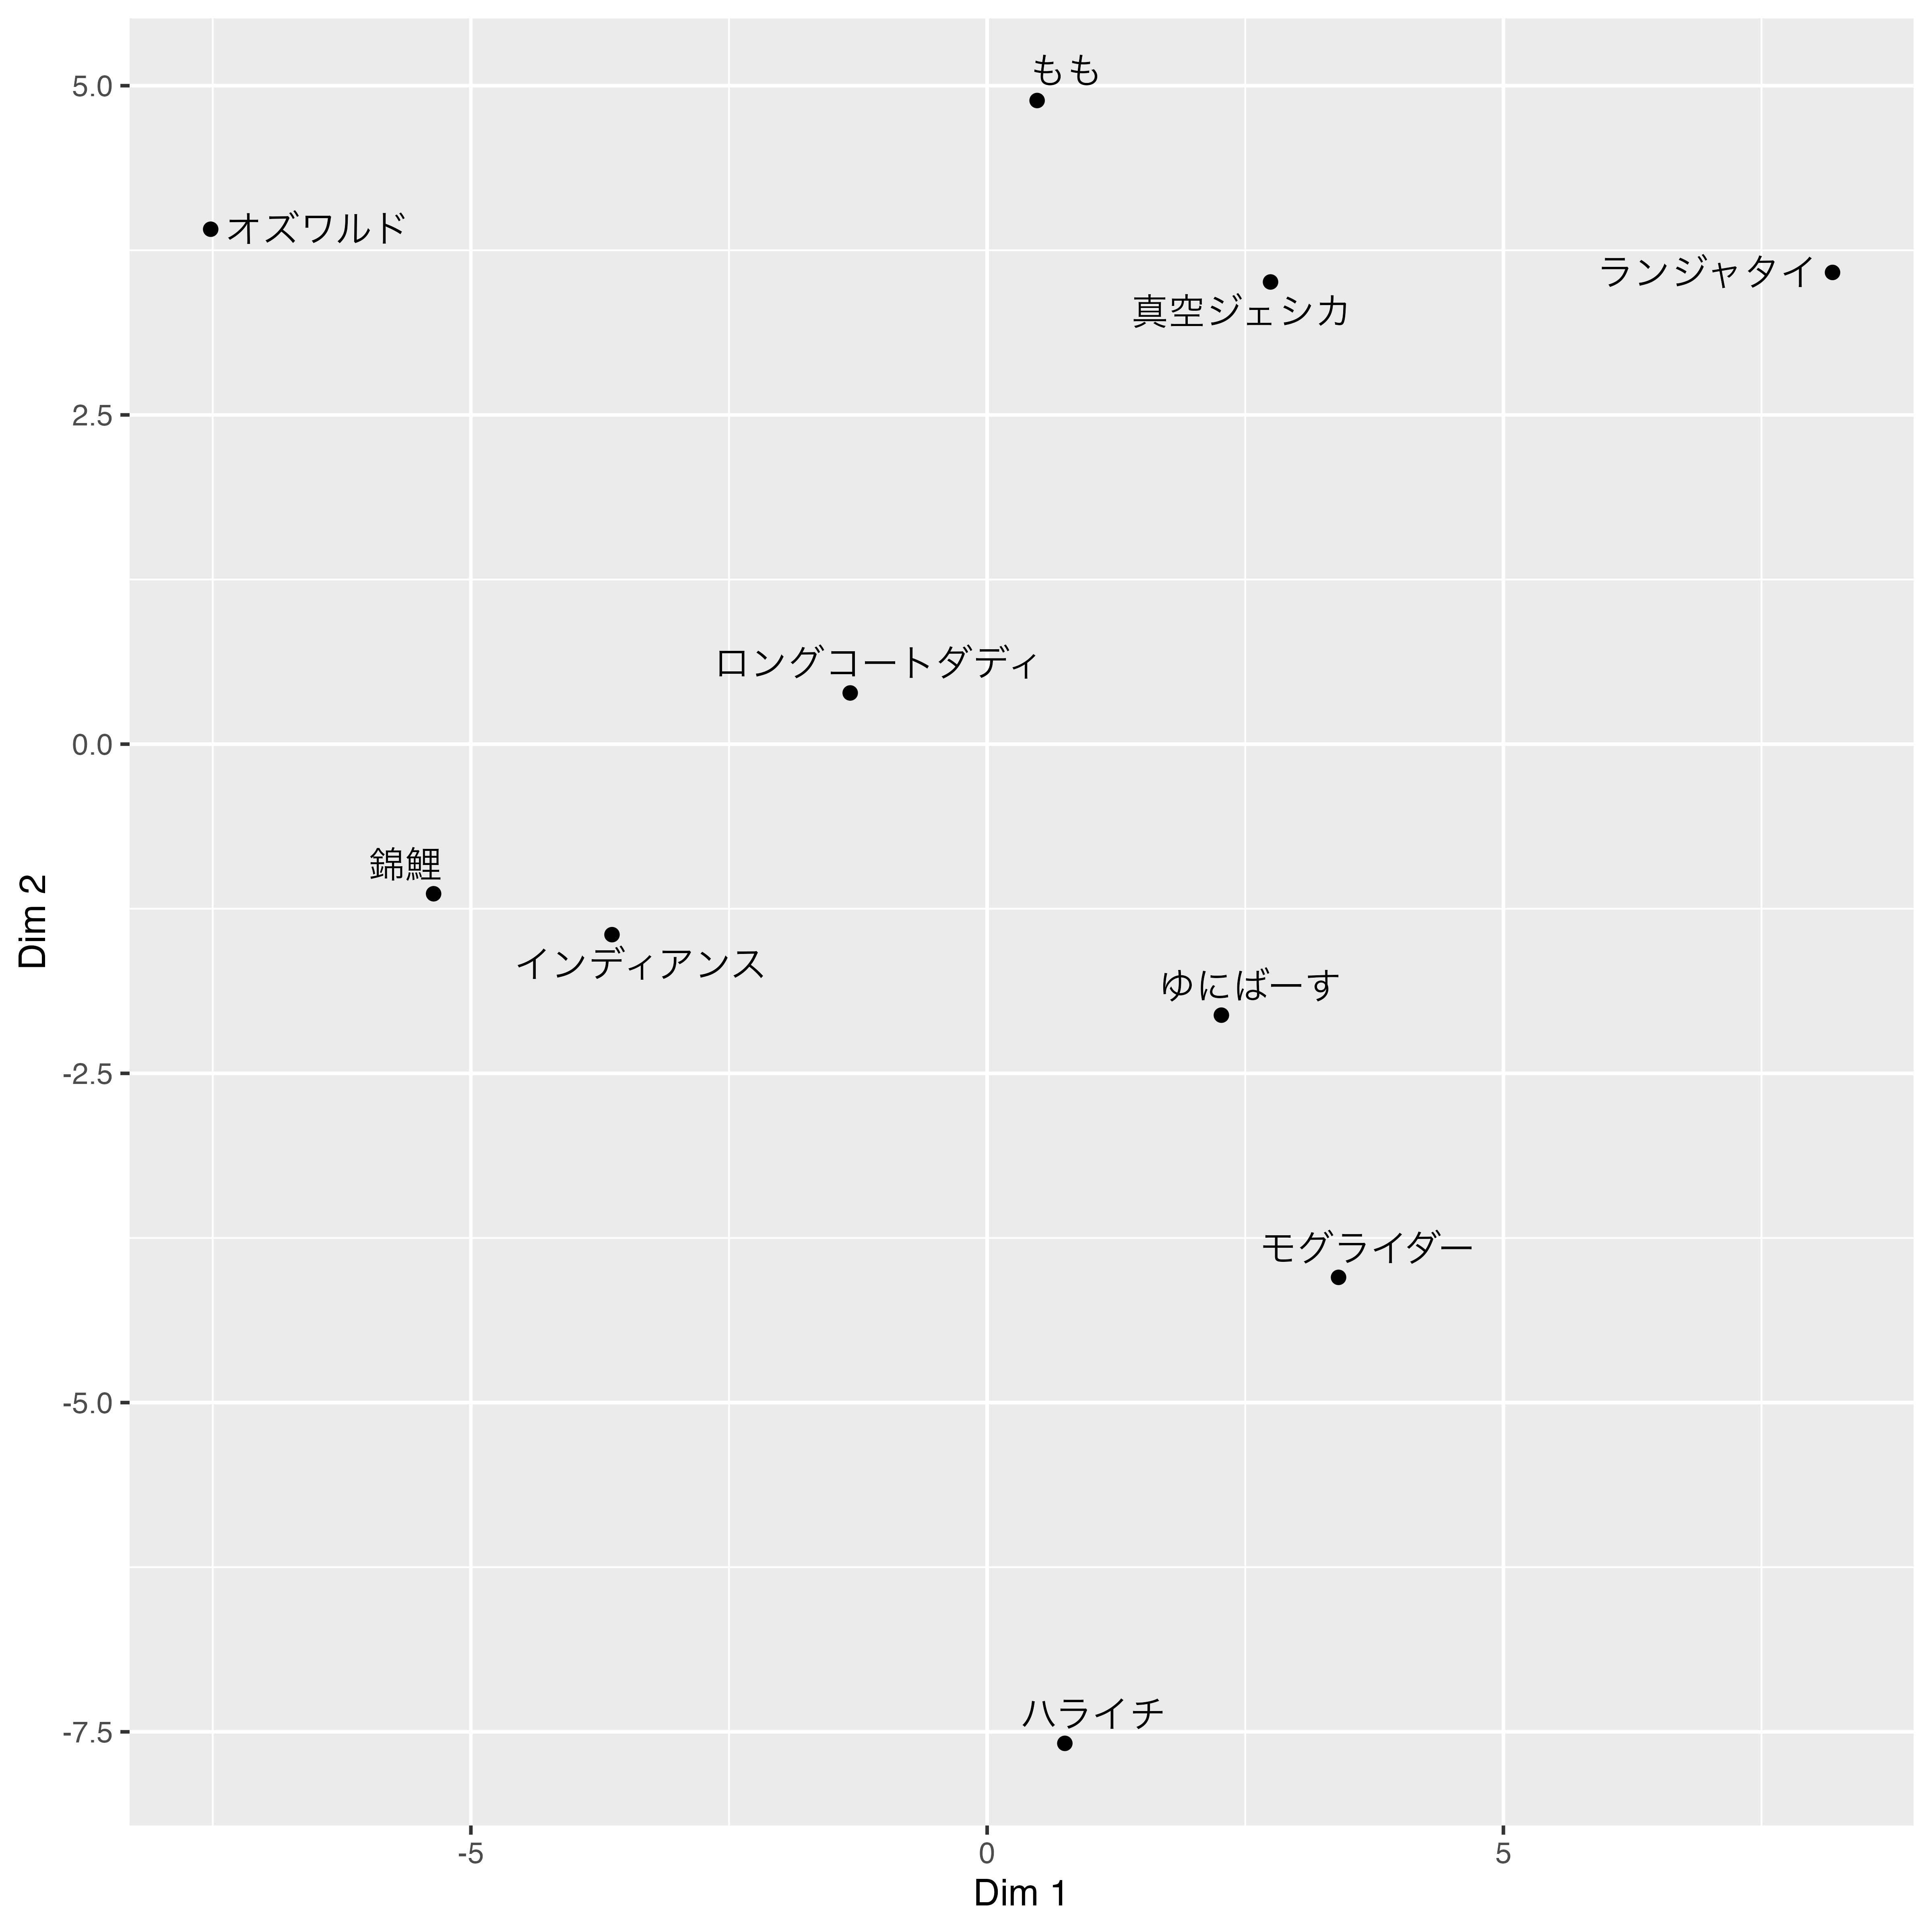
\includegraphics[width=0.8\linewidth,keepaspectratio]{../images/Rplot15_03.png}
		\caption{非計量MDSのプロット}
		\label{fig::15_03}
	\end{center}
\end{figure}

またMDSでは，地図を書くことはできても東西南北を固定することはできませんから，因子分析のように軸の解釈をすることはあまりありません。しかし座標を説明変数として，外的な被説明変数に回帰分析をすることで，軸が何を反映しているのかを考えることができます。これについては\textcite{kosugi2016a}のMDSの章を参照してください。あるいは，MDSの結果と同じデータのクラスター分析の結果を組み合わせて考察することもあります。

このように，非計量MDSは優劣・大小関係という順序尺度水準の評定だけからでもその空間的な特徴を描くことができますから，心理尺度のもつ仮定や測定モデルを考える必要がないため，今後その重要性が再発見されていくのではないかと思います。しかしMDSの面白さはこれだけにとどまりません。測定論的にも方法論的にも，大きな可能性を秘めた応用モデルが考えられています。

\section{MDSの応用モデル}
\subsection{個人差多次元尺度構成法}
MDSはある個人が主観的に判定した距離行列からでも，地図を書くことができます。ある人に，「ハライチとランジャタイは(芸風が)似てると思う?」などと聞いて数字で答えさせ，距離行列を作って非計量MDSで分析すれば，その人の心の中でお笑い芸人をどのように分類しているかを見ることができるわけです。心理尺度をわざわざ構成しなくても，ある人の感覚を数量的に表現してその大小関係が妥当なものであるならば，その人の心の中での配置がわかるのです。個人の内部状態を個人の基準で判断させるような研究においては，既に指摘したような心理尺度の理論的根拠の弱さは該当しませんから，目的によってはMDSの方がよほど適しているはずです。

しかし気になることがあるとすれば，個々人の心の状態がわかるのは良いにしても，それではケースバイケース，つまり「この人の中ではこうなっているようだ」という限定的な言及しかできないのが苦しいところです。心理学は曲がりなりにも，人間一般の行動なり感覚なりを研究したいわけですから，人生いろいろ，の一言で終わらせてしまうわけにはいかないのです。

でも大丈夫。個人差を踏まえてMDSを考える，つまり二相三元データを分析するMDSの方法も，古くから研究されています。もっとも有名なモデルのひとつが\textcite{carroll1970analysis}による\keytermL{INDSCAL}{INDSCAL}(INdividual Differences SCALing,個人差多次元尺度構成法)\footnote{これの発音は「インスカル」です。``D''は読まないことに注意。}です。

個人$i$が対象$j$と$k$に対して与えた類似度を$\delta_{jk}^i$と表すとしましょう。個人$i$にかかわらず，全体的には$p$次元空間において
\[ d_{jk} = \sqrt{\sum_{t=1}^p (x_{jt}-x_{kt})^2} \]
という関係で表現されているとし，個人差を
\[ d_{jk}^i = \sqrt{\sum_{t=1}^p w_{it}(x_{jt}-x_{kt})^2} \]
として表現します。つまり第$t$番目の次元に個々人の重み$w_{it}$があるとモデル化し，「人によって重視する次元がある」と考えるのです。モデルの推定にあたっては，$w_{it}\gt 0$と$\sum_t w_{it}^2=1$などの制約を課します。

さて図\ref{INDSACLimage}には共通次元のプロットと個人A,Bごとの強調パターンを示しました。図中のX1,X2,X3,X4が共通次元のプロットを表しています。個人Aは第一次元に重みを持つ人の例で，X1,2,3,4がA1,2,3,4のように左右に広がって布置されています。
個人Bは第一次元に1.0未満の，第二次元に1.0以上の重みを持つ人の例で，B1,2,3,4のように第一次元を短く，第二次元を大きく拡張しています。一般的なX1-X3の距離に比べて，Aはその両者の違いが大きいと判断し，Bはその違いが小さいと判断しているわけです。つまりAは第一次元の方向に敏感で，Bは鈍感である，といった解釈をすることができます。


\begin{figure}[ht]
	\begin{center}
		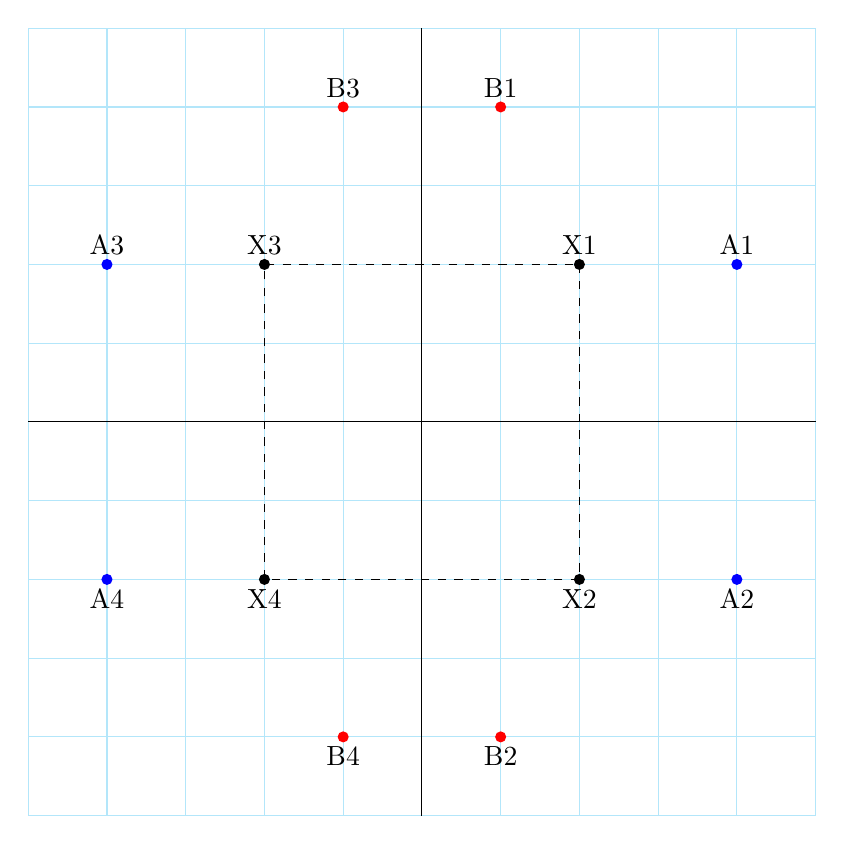
\begin{tikzpicture}
			\draw [cyan!30] (-5,-5) grid (5,5);%"細線の方眼"
			\draw[-] (-5,0)--(5,0); %x軸
			\draw[-] (0,-5)--(0,5); %y軸
			\coordinate (X1) at (2,2);
			\coordinate (X2) at (2,-2);
			\coordinate (X3) at (-2,2);
			\coordinate (X4) at (-2,-2);
			\fill (X1) circle [radius=2pt];
			\fill (X2) circle [radius=2pt];
			\fill (X3) circle [radius=2pt];
			\fill (X4) circle [radius=2pt];
			\draw[dashed](X1)--(X2)--(X4)--(X3)--(X1)--cycle;
			\node[above] at (X1) {X1};
			\node[below] at (X2) {X2};
			\node[above] at (X3) {X3};
			\node[below] at (X4) {X4};
			\coordinate (A1) at (4,2);
			\coordinate (A2) at (4,-2);
			\coordinate (A3) at (-4,2);
			\coordinate (A4) at (-4,-2);
			% \draw[->] (A1)--(4.5,2);
			% \draw[->] (A2)--(4.5,-2);
			% \draw[->] (A3)--(-4.5,2);
			% \draw[->] (A4)--(-4.5,-2);
			\fill[blue] (A1) circle [radius=2pt];
			\fill[blue] (A2) circle [radius=2pt];
			\fill[blue] (A3) circle [radius=2pt];
			\fill[blue] (A4) circle [radius=2pt];
			\node[above] at (A1) {A1};
			\node[below] at (A2) {A2};
			\node[above] at (A3) {A3};
			\node[below] at (A4) {A4};
			\coordinate (B1) at (1,4);
			\coordinate (B2) at (1,-4);
			\coordinate (B3) at (-1,4);
			\coordinate (B4) at (-1,-4);
			\fill[red] (B1) circle [radius=2pt];
			\fill[red] (B2) circle [radius=2pt];
			\fill[red] (B3) circle [radius=2pt];
			\fill[red] (B4) circle [radius=2pt];
			\node[above] at (B1) {B1};
			\node[below] at (B2) {B2};
			\node[above] at (B3) {B3};
			\node[below] at (B4) {B4};
		\end{tikzpicture}
		\caption{INDSCALによる軸の協調イメージ}
		\label{INDSACLimage}
	\end{center}
\end{figure}

このように，INDSCALを使えば個人の判断次元の重要度をその重みとして表現することができます。ただのMDSと違ってINDSCALは軸の回転に対して不定性をもっていますから，それぞれの軸がどういう意味であるかを解釈することができます。何より，全体の特徴だけでなく個人差をモデルの中に表現することができることは，心理学の研究用途にとって非常に有用な特徴ではないでしょうか。

より慎重に考えるならば，この個人差の表し方は「個々人で原点が同じ」であり，「次元の重みが個人差である」という仮定を置いていることになります。第\ref{H06_Attitude}章で心理尺度の問題として，個々人の評定をどのように合算するのかについて理論的根拠がない，という批判をしました。これについてINDSCALではこのような仮定でモデル化する，としているだけで，理論的根拠を示すものではありません。しかし，モデルの形で個人間の取り扱いを明示していることは，しばしばその存在にすら気づかれない水面下の仮定をとるよりも，建設的な議論を可能にします。もし個人差の表し方，個人間の表現に疑義があるのであれば，心理学者も積極的に三相データのモデル化に取り組むべきでしょう。

\subsection{展開法}
ここまでは距離データとして，直接的に変数間の距離が測定されたものとして考えられてきました。つまり一相二元のデータから分析が始まっており，一般的な個人$\times$変数の二相二元のデータセットがあった場合は，いずれかの相を潰して分析しなければなりません。
これに対して\textcite{coombs1950psychological}は，刺激に対する個人の選好順位から一次元尺度を作る\keyterm{展開法}{てんかいほう}{Unfolding method}を提案しました。この方法では，個人$\times$変数の組み合わせで得られるデータを，両者の距離と考えるところがポイントあり，態度尺度作成法の一つとしても考えられてきました\parencite{Fujihara2001}。ある態度対象$A_j$，たとえば政治的態度であれば「自民党」「共産党」などですが，これに個人$i$が選好順序をつけたとします。自分は自民党のほうが共産党より好きだ，といった感じです。これは個人$i$と態度対象$A_j$の距離を表していると考えられます。この距離に応じて，態度対象が一次元上に並んでいると考えるのです。態度対象が並んでいる連続体をJ-Scaleといいます。もちろん人によって選好度は異なります。別の人にとっては共産党のほうが自民党より好きだ，となることもあるのです。こうした個人の違いは，J-Scale上の個人の立ち位置が違うのであって，個人の尺度は態度と垂直する方向に伸びていると考えます。個々人の尺度をI-Scaleといいますが，この尺度はJ-Scaleを個人の位置で折り畳んだものになっていると考えるのです。

図\ref{Unfolding1}には，4つのカテゴリをもつJ尺度と，個人$i,k$のI尺度を示しました。個人のJ尺度上の理想点$IP_i,IP_k$の上に各カテゴリがたたみ込まれており，表に出てくるときはこれが展開すると考えるわけです。
\begin{figure}[ht]
	\begin{center}
		\begin{tikzpicture}
			\draw[-] (-3,0)--(6,0) node[below,right] {J-Scale}; %x軸
			\coordinate (X1) at (-2,0);
			\coordinate (X2) at (0.5,0);
			\coordinate (X3) at (2,0);
			\coordinate (X4) at (4.2,0);
			\fill (X1) circle [radius=2pt];
			\fill (X2) circle [radius=2pt];
			\fill (X3) circle [radius=2pt];
			\fill (X4) circle [radius=2pt];
			\node[above] at (X1) {A1};
			\node[above] at (X2) {A2};
			\node[above] at (X3) {A3};
			\node[above] at (X4) {A4};
			\draw[-] (-1,0) -- (-1,-6) node[below,right]{I-Scale};
			\draw[-] (3.5,0) -- (3.5,-6) node[below,right]{I-Scale};
			\node[above] at (-1,0) {$IP_k$};
			\node[above] at (3.5,0) {$IP_i$};
			\coordinate (i1) at (-1,-1);
			\coordinate (i2) at (-1,-1.5);
			\coordinate (i3) at (-1,-3);
			\coordinate (i4) at (-1,-5.2);
			\fill[cyan!30] (i1) circle [radius=2pt];
			\fill[cyan!30] (i2) circle [radius=2pt];
			\fill[cyan!30] (i3) circle [radius=2pt];
			\fill[cyan!30] (i4) circle [radius=2pt];
			\draw[dashed,bend left = 280] (X1) to (i1);
			\draw[dashed,bend left = 30] (X2) to (i2);
			\draw[dashed,bend left = 30] (X3) to (i3);
			% \draw[dashed] (X4) -- (i4);
			\coordinate (k1) at (3.5,-0.7);
			\coordinate (k2) at (3.5,-1.5);
			\coordinate (k3) at (3.5,-3);
			\coordinate (k4) at (3.5,-5.5);
			\fill[blue!30] (k1) circle [radius=2pt];
			\fill[blue!30] (k2) circle [radius=2pt];
			\fill[blue!30] (k3) circle [radius=2pt];
			\fill[blue!30] (k4) circle [radius=2pt];
			\draw[dashed,bend left = 290] (X3) to (k2);
			\draw[dashed,bend left = 30] (X4) to (k1);
			% \draw[dashed] (X3) -- (k2);
			% \draw[dashed] (X4) -- (k1);
		\end{tikzpicture}
		\caption{展開法による一次元尺度の構成}
		\label{Unfolding1}
	\end{center}
\end{figure}



これを多次元に拡張したモデルもあります。多次元展開法は，$p$次元空間における個人の理想点$P_i$と，態度対象の布置$A_j$との距離$d(P_i,A_j)$を次のように考えます。
\[ d(P_i,A_j) = \sqrt{\sum_{t=1}^p (P_{it} - A_{jt})^2} \]
さらに，個人$i$が態度対象$j$に対して「4.かなり当てはまる」とか「1.全く当てはまらない」などと評価するわけですが，この評価$R_{ij}$が構成される多次元空間上の距離の関数になっている，すなわち
\[ R_{ij} = \alpha - \beta d(P_i,A_j) \]
と考えます。ここで一次関数的に表現していることから，モデル上の距離と評定値との残差を最小にするような定数(回帰係数)として$\alpha,\beta$を求めるということです。

展開法はRの\verb|smacof|パッケージなどでも実行できるようになっています。

この方法のポイントは，個人と態度対象を同じ空間に埋め込み，その座標を考えることにあります(図\ref{Unfolding2})。評定値が尺度によるスコアと考えるのではなく，態度対象との距離関係を表しているものとみなして分析するわけです。リッカート的なスコアリングは，1,2,3...と振られる数字が大きくなるにつれて，その態度の強度が累積的に大きくなっていくことを含意しています。態度とはそのような強度を持つものである，という仮定があり，測定しているのが態度であれば問題ないのですが，リッカート法が必ずしも社会的態度だけでなくそれ以外のものも測定するのに用いられている現状を顧みるに，その数字が何を表しているのかについて別の角度から考えるのも，これからの心理測定のヒントになるかもしれません。
\begin{figure}[ht]
	\begin{center}
		\begin{tikzpicture}
			\draw[-] (-1,0)--(6,0); %x軸
			\draw[-] (-0.5,-1)--(-0.5,6); %y軸
			\clip (-1,-1) rectangle (6,6);
			\coordinate (A1) at (1.5,4);
			\coordinate (A2) at (4,2);
			\coordinate (S1) at (1,1);
			\coordinate (S2) at (4.2,3);
			\fill[red] (A1) circle [radius=2pt];
			\fill[red] (A2) circle [radius=2pt];
			\fill[blue] (S1) circle [radius=2pt];
			\fill[blue] (S2) circle [radius=2pt];
			\node[above] at (A1) {A1};
			\node[below] at (A2) {A2};
			\node[below] at (S1) {S1};
			\node[above] at (S2) {S2};
			\draw[<->] (S1) -- (A1) node[midway,left]{$d(P_1,A_1)$};
			\draw[blue,dashed] (S2) circle [radius=1];
			\draw[blue,dashed] (S2) circle [radius=2];
			\draw[blue,dashed] (S2) circle [radius=3];
		\end{tikzpicture}
		\caption{多次元展開法による態度対象と個人の同時プロット。個人S2は態度対象A1よりA2のほうに近い}
		\label{Unfolding2}
	\end{center}
\end{figure}
\subsection{非対称多次元尺度構成法}
MDSの応用例として最後にご紹介するのは，非対称多次元尺度構成法です。距離とは対称性，すなわち$d(x,y)=x(y,x)$という性質を満たすものですが，この条件を取り払ったものを考えます。

たとえば親近性のように，AさんがBさんのことを好きだと思っていても，BさんはAさんのことが嫌いである，といった非対称性は人間関係ではザラにあることです。このほかにも，日本から米国への輸出量と，米国から日本への輸出量(日本の米国からの輸入量)が異なるとか，地方から東京への人口移動とその逆といったことも，対象間の非対称性の例です。あるいはビールから発泡酒に変える人はいるけど，逆の人は少ない，といった購買行動におけるブランドスイッチングなども非対称関係が見られます。こうした非対称な情報が測定の誤差でないとするならば，何らかの意味が読み取れるように分析しなければなりません。それを考えるのが非対称多次元尺度構成法です。

\subsubsection{地図に加筆するモデル}
MDSは他の多変量解析と違って，非対称関係を考えることができるだけでなく\footnote{たとえば分散共分散行列や相関行列は，その行列計算の手続きの中でどうしても正方対称行列になってしまいますから，非対称関係を表現することができません。}，地図を描いているわけですからその地図に情報を書き足すなど，表現上の工夫で対応することもできます。

非対称な関係を地図上に表された対象に書き加えるモデルは，基本的に非対称データを対称部と歪対称部に分割します。すなわち非対称行列$\bm{S}$に対して，次のような変換をします。
\[ \bm{S} = s_{jk} = \frac{1}{2}(\bm{S}+\bm{S}') + \frac{1}{2}(\bm{S}-\bm{S}')= \bm{S}_s + \bm{S}_{sk} \]
これは要するに平均をとったところと，そこからのずれのところに分割するようなもので，数値例を見るとすぐにお分かりいただけると思います。
\[ \begin{pmatrix} 0 & 4 & 1 & 3 \\
                1 & 5 & 1 & 2 \\
                2 & 2 & 5 & 4 \\
                3 & 3 & 7 & 5\end{pmatrix} =
	\begin{pmatrix} 0.0 & 2.5 & 1.5 & 3.0 \\ 2.5 & 5.0 & 1.5 & 2.5 \\ 1.5 & 1.5 & 5.0 & 5.5\\3.0 & 2.5 & 5.5 & 5.0 \end{pmatrix}
	+
	\begin{pmatrix} 0.0 & +1.5 & -0.5 & 0.0 \\ -1.5 & 0.0 & -0.5 & -0.5 \\ +0.5 & +0.5 & 0.0 & -1.5 \\ 0.0 & +0.5 & +1.5 & 0.0 \end{pmatrix}
\]
このように考えると，前半の対称部$\bm{S}_s$については一般的なMDSを施すことができます。これで布置が得られたら，その周りに非対称情報を書き加えれば良いのです。
たとえばOkada-Imaizumiモデル\parencite{okada1987nonmetric,okada1997asymmetric}では，歪対称な情報を円または楕円で表現します。
2点間の距離$r_{jk}$は，対称な距離$d_{jk}$に加えて，点j,kがまとう楕円の半径$r_j,r_k$を使って，
\[ r_{jk} = d_{jk} -r_j + r_k \]
とします。両者の点間距離$d_{jk}$から出発点の半径を引く，つまり円の外縁からスタートし，到達点の半径を足す，つまり円の外縁までを距離として表現するのです。
\begin{figure}[ht]
	\begin{center}
		\begin{tikzpicture}
			\coordinate (J) at (0,0);
			\coordinate (K) at (5,0);
			\coordinate (rj1) at (0,3);
			\coordinate (rj2) at (2,3);
			\coordinate (djk) at (6,3);
			\coordinate (rk1) at (6,-3);
			\coordinate (rk2) at (5,-3);
			\coordinate (dkj1) at (4,-3);
			\coordinate (dkj2) at (-2,-3);
			\coordinate (djk1) at (5,-5);
			\coordinate (djk2) at (0,-5);
			\fill (J) circle [radius=2pt];
			\fill (K) circle [radius=2pt];
			\node[below left] at (J) {j};
			\node[above right] at (K) {k};
			\draw (J) circle [radius=2];
			\draw (K) circle [radius=1];
			\draw (-2,0) -- (6,0);
			\draw[dashed] (rj1) -- (J);
			\draw[dashed] (rj2) -- (2,0);
			\draw[dashed] (6,0) -- (djk);
			\draw[dashed] (6,0) -- (rk1);
			\draw[dashed] (K) -- (rk2);
			\draw[dashed] (4,0) -- (dkj1);
			\draw[dashed] (-2,0) -- (dkj2);
			\draw[dashed] (J) -- (djk2);
			\draw[dashed] (K) -- (djk1);
			\draw[<->] (rj1) -- (rj2) node[midway,above]{$r_j$};
			\draw[<->] (rj2) -- (djk) node[midway,above]{$r_{jk}$};
			\draw[<->] (rk1) -- (rk2) node[midway,above]{$r_k$};
			\draw[<->] (dkj1) -- (dkj2) node[midway,above]{$r_{kj}$};
			\draw[<->] (djk1) -- (djk2) node[midway,above]{$d_{kj}$};
		\end{tikzpicture}
		\caption{Okada-Imaizumiモデルによる非対称関係の表現}
		\label{OImodel}
	\end{center}
\end{figure}
各点がまとう円のサイズは違いますから，$j \to k$と$k \to j$の距離がその半径分プラスマイナスされることで非対称な関係として表すことができます。また図\ref{OImodel}は円を書き加えましたが，次元ごとに重みが違う楕円で表現することもできます\footnote{\textcite{fujisawaCore}の付録にはソシオメトリックデータにこのモデルを応用した例が掲載されています。}。

円や楕円を纏うだけでなく，全体的に非対称性を持っている方向に矢印や確率分布を纏わせるモデル\footnote{\textcite{Shojima2011}は，空間統計学で用いられるフォン・ミーゼス分布を点の周りに纏わせる，非対称フォン・ミーゼス尺度法を提案しています。}，空間に風向きや勾配などで非対称関係を表現するモデルなど，色々なものが提案されています。

これらはいずれも，地図の上に別の情報を追加するというアイデアからきています。MDSで描画されたものが地図ですから，その上に別の情報を載せることでほかにもさまざまな表現ができるかもしれませんね。
\subsubsection{数学的に展開したモデル}
\textcite{Chino2012}は非対称MDSを網羅的にまとめていますが，彼の提案する\keyterm{エルミート形式モデル}{えるみーとけいしきもでる}{Hermitian Form Model}はさまざまな非対称MDSモデルの中でも，数学的な拡張でもって非対称情報の描画を考えた野心的なモデルであると言えます。

非対称行列$\bm{S}$を対称部$\bm{S}_s$と歪対称部$\bm{S}_{sk}$に分解するところまでは同じなのですが，歪対称部を虚数で表す，つまり
\[ \bm{H} = \bm{S} + i\bm{S}_{sk} \]
とすることで，非対称行列を複素数で表現することを考えます。複素数の世界\footnote{念のために書いておきますが，複素数とは$i=\sqrt{-1}$となるような虚数単位を導入し，実部と虚部の和，すなわち$a+bi$のかたちで一つの数字を表現する方法です。}において，虚部の符号が違うだけのもの，すなわち$a + bi$に対する$a - bi$は特に共役複素数と呼びます。非対角要素に共役複素数が入っている行列は，複素数の世界からみれば対称行列のような性質を持っており，特に\keytermL{エルミート行列}{えるみーとぎょうれつ}と呼ばれてその性質が研究されています。

非対称行列は固有値分解すると，固有値も固有ベクトルも複素数で得られるのですが，エルミート行列になっていると固有値は実数になります。固有ベクトルは複素数になりますが，計量MDSの時にみたように固有ベクトルが複素空間における座標として，また要素同士の内積が両者の距離として考えることができます。そもそも対称行列を実数の空間にプロットすることが難しいのが非対称行列を扱う上での問題だったわけですが，プロットする空間の方を複素空間に拡張することで，数学的に自然な形でMDSを展開することができるのです。\textcite{kosugi2004}ではこのモデルを社会心理学におけるバランス理論に応用しています。

HFMは分析の元になるデータが計量的，すなわち間隔尺度水準以上であることが求められます。心理学の応用的側面としては，比率尺度水準以上のデータを入手することが困難かもしれませんが，複雑な人間関係などを線形関係や実数の中だけで理解するのはそもそも難しいかもしれません。複素数を扱った心理学理論など，考えてみるのも面白いかもしれませんね。



\end{document}